\scanpage{15}
un hom d'Algèbres graduées
\[
\operatorname{Symm}\underline E\longrightarrow(\operatorname{Symm}E)_{(p)}
\]
(degrés multipliés de $p$)

Le \deleted{\unsure{f}} faisceau inverse de
$\underline{\mathcal O}_{\underset{\sim}{\mathrm P}(p_S(\underline E))}(1)$ est
$\underline{\mathcal O}_{\underset{\sim}{\mathrm P}(\underline E)}(p)$.
\unsure{Le noter. cas plus général}.

Si $\unsure{\underline L|\underline E}$ est un Module \uline{inversible}, on a un
\uline{isom canonique}
\[
p(\underline L)\simeq\underline L^{\otimes p}.
\]
\margin{Exemple : $\underline E=\mathcal O_S^n$, d'où
$\deleted{p_S(\unsure{\mathrm V}(\underline E))}p_S(\underline E)\simeq\mathcal O_S^n$, donc
$p_S(S[t_1,\ldots,t_n])\simeq S[t_1,\ldots,t_n]$, l'hom canonique
défini par $t_i\rightsquigarrow t_i^p$.
Si on a un sous-schéma de $\underline E$ défini par des équations,
on élève les \uline{coefficients} de ces équations à la puissance \unsure{$p$ième}.
Analogue pour des équations homogènes, \unsure{et} définissant un schéma projectif.}
\figure{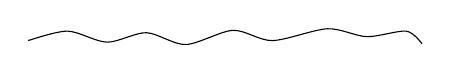
\begin{tikzpicture}\draw plot[smooth] coordinates {(0,0) (.5,.12) (1,-.02) (1.5,.1) (2,-.05) (2.6,.13) (3.1,0) (3.8,.15) (4.3,.05) (4.8,.12) (5,-.04)};\end{tikzpicture}}

Changement de base des Frobenius

\deleted{[cf diagramme]}

1°) (cf diagramme)
\[
\unsure{P_X|p_X}(X')\simeq p_S(X')\times_{p_S(X)}(X,\operatorname{Frob}_S(X)):
\]
et avec cette identification, \deleted{\unsure{un}}
$\operatorname{Frob}_X(X')$ est défini de façon évidente par
$\operatorname{Frob}_S(X')$ et $\operatorname{Frob}_S(X)\circ g$.

2°) Si on a un chgt de base $S'\mathbin{\text{---}}S$, on a
\[
p_S(X)\times_S S'\simeq p_{S'}(X\times_S S')
\]
Cet isom étant fonctoriel en $X$, \deleted{\unsure{et le foncteur}}
\inserted{\unsure{le foncteur chgt}}
\unsure{l'hom de ch. de base} transforme $\operatorname{Frob}_S(X)$ en
$\operatorname{Frob}_{S'}(X\times_S S')$.
\mspage{14}
